\section{Quantifying uncertainty on Excursion Sets implicitly defined by Gaussian processes}
\label{sec:ESEP}

We define the random sets of interest in Section \ref{sec:ES}, while the closed-form expressions for the expected uncertainty reduction are derived in Section \ref{sec:EIBV}. Section \ref{Sec:UnivarEx} provides an instructive bivariate example relevant for sampling in the temperature and salinity application.

\medskip

Our objective is to leverage statistical tools onboard an autonomous
robotic platform to characterize a river plume, focusing on spatial
separation of cold freshwater from a river and warmer saline waters
of a fjord.

In order to formalize the problem in mathematical terms, let us
consider a multivariate (i.e., vector-valued) Gaussian random field
$(\gp[\x])_{\x \in \mathcal{M}}$, where $\mathcal{M}$ is an arbitrary
set and the dimensionality of the output $\no \geq 1$ is arbitrary.

Assume furthermore that the set of interest
is characterized in terms of a subset of values of the response variables, say
$\T \subset \R^{\no}$, and denote the corresponding set of spatial locations by
$$
\es=\gp^{-1}(\T)=\{\x \in \mathcal{M}: \gp[\x] \in \T\}.
$$
Our goal here is to develop approaches to quantify and improve the
characterization of uncertainties on such sets $\es$, in the
context of multivariate random fields.

While some aspects of the developed approaches do not call for a
specific form of $\T$, we will often stick for simplicity to the case
of orthants
($\T=(-\infty, t_1] \times \dots \times (-\infty, t_{\no}]$ where
$t_1,\dots, t_{\no} \in \R$) as this will allow efficient calculation
of several key quantities. Note that changing some $\leq$ inequalities
to $\geq$ ones would lead to immediate adaptations.

If we assume that $\gp$ has
continuous trajectories (almost surely) and $T$ is closed, then
$\es$ becomes a Random Closed Set
\citep{Molchanov2005}. %In what follows, we will express various quantities related to $\es$ in terms of $\gp$'s moments both for general and orthant $T$'s.
\textcolor{red}{Peut etre supprimer } In what follows, we will be interested in characterizing the distribution of the volume of the excursion set $\es$ with respect to some (locally finite, Borel) measure $\mes$
on $D$.

\subsection{Background and Notation}
\subsubsection{Co-kriging with respect to (batches) of generalized locations}

To keep things as general as possible, we will consider performing measurements
in batches, i.e. collecting several observations at a time. Moreover, we assume
that given a site $s\in D$, one can choose which component(s) of
$\gp[s]\in\mathbb{R}^{\no}$ one wants to observe.
%observation of several components at a time being also allowed. 
Denoting here for  $s\in D$ and $\ell \in \{1\dots,p\}$ the $\ell\text{th}$ component of $\gp[s]$ by $\gp[s,\ell]$ or 
$\gp[x]$ with $x=(s,\ell)$, we see that $Z$ can actually also be thought of as a scalar-valued Gaussian random field 
indexed by $D\times \{1\dots,p\}$. This simple change of representation allows in turn revisiting cokriging as kriging 
in extended index set, and hence enjoying kriging results (such as batched-sequential update formulae, tackled in
the next section) without unneccesary complications.
%
Let us refer to $x=(s,\ell)$ as (generalized) location and use boldface $s, \ell, x$ to denote batches of sites, 
response indices, and generalized locations, respectively. A batch $\bm{x}=(x_1,\dots, x_q)$ of generalized locations 
with $x_i=(s_i,\ell_i)$ $(1\ldots i \ldots q)$ is also by a slight abuse oftentimes denoted $\bm{x}=(\bm{s}, \bm{\ell})$ 
for convenience.
%
We will also use concatenation for the field evaluated at a batch of generalized locations
\begin{align*}
\gp[\bm{x}]:=
\left(\gp[s_1,\ell_1], ...,
\gp[s_q,\ell_{q}]\right) \in \mathbb{R}^{q}.
\end{align*}
%
Assuming now that $n$ batches of observations are available, with respective sizes $q_1,\dots, q_n$, and that one wishes 
to predict $\gp[\bm{x}]$ for some batch of $q\geq 1$ generalized locations $\bm{x}=(\bm{s}, \bm{\ell})$, the (simple) 
cokriging mean would then amount to simple kriging with respect to a scalar-valued Gaussian random field indexed by 
$D\times \{1\dots,p\}$ and with covariance kernel $k(\bm{x}, \bm{x}')=K(\bm{s}, \bm{s}')_{\ell, \ell'}$, that is:
%
\begin{equation}
\mu_{[n]}(\bm{x})=\mu(\bm{x})+\lambda_{[n]}(\bm{x})^T (\mathbf{z}_{[n]}-\mu(\bm{x})),
\end{equation}
where $\mu$ is $Z$'s initial mean function, $\mathbf{z}_{[n]}$ stands for the ($\sum_{i=1}^n q_i$)-dimensional vector of 
observed responses of $Z$ at all considered generalized locations, and $\lambda_{[n]}(\bm{x})$ is a vector of weights 
equal to $k(\bm{x}_{[n]}, \bm{x}_{[n]})^{-1} k(\bm{x}_{[n]}, \bm{x})$ with $\bm{x}_{[n]}=(\bm{x}_1,\dots, \bm{x}_n)$, 
$k(\bm{x}_{[n]}, \bm{x}_{[n]})$ being assumed non-singular throughout the presentation. The co-kriging %(conditional) 
residual (cross-)covariance function (with respect to batches of generalized locations) can also be expressed in the same vein via
%
\begin{equation}
k_{[n]}(\bm{x},\bm{x}')=k(\bm{x},\bm{x}')-\lambda_{[n]}(\bm{x})^T k(\bm{x}_{[n]}, \bm{x}_{[n]}) \lambda_{{[n]}}(\bm{x}').
\end{equation}

\subsubsection{Co-kriging update formulae}

Let us now consider the case where co-kriging prediction of $Z$ was made with respect to $n$ batches $\bm{x}_i$ of generalized locations, concatenated again within
$\bm{x}_n=(\bm{x}_1,\dots, \bm{x}_n)$, and one wishes to update the prediction by incorporating a new vector of observations $\mathbf{z}_{n+1}$ measured at a batch of $q_{n+1} \geq 1$ generalized locations $\bm{x}_{n+1}$.
%It turns out that the concept of \textit{generalized location} makes the kriging formulae form-invariant across all dimensions. This allows us to directly adapt the 
Thanks to our representation of co-kriging in terms of simple kriging with respect to generalized locations, a strightforward adaptation of the batch-sequential kriging update formulae from \cite{Chevalier.etal2013a} delivers that
% 
\begin{equation}
\mu_{[n+1]}(\bm{x})=\mu_{[n]}(\bm{x})+\lambda_{[n+1,n+1]}(\bm{x})^T (\mathbf{z}_{n+1}-\mu(\bm{x}_{n+1})),
\end{equation}
where $\lambda_{[n+1,n+1]}(\bm{x})$ denotes the $q_{n+1}$-dimensional sub-vector extracted from
$\lambda_{[n+1]}(\bm{x})$ that corresponds to the kriging weigths associated with the last $q_{n+1}$ responses when 
predicting at $\bm{x}$ relying on all measurements until batch $(n+1)$.
%\text{th}$ batch.
%, i.e. those from the $(n+1)\text{th}$ batch of measurements conducted at $\bm{x}_{n+1}$.
Similarly, the updated co-kriging residual (cross-)covariance function then writes
\begin{equation}
k_{[n+1]}(\bm{x},\bm{x}')=k_{[n]}(\bm{x},\bm{x}')-\lambda_{[n+1,n+1]}(\bm{x})^T k_{[n]}(\bm{x}_{[n]}, \bm{x}_{[n]}) \lambda_{{[n+1,n+1]}}(\bm{x}').
\end{equation}
%\medskip
%
Let us remark that, as noted in \cite{Chevalier2015} in the case of scalar-valued fields, these update formulae naturally 
extend to Universal Kriging in second-order settings and apply without Gaussian assumption. We will now see how the latter formulae are instrumental in deriving semi-analytical formulae for stepwise uncertainty reduction criteria for 
vector-valued random fields.



\subsection{UQ on ES of vector-valued fields with volume moments and friends (focus on VV and IBV)}
We now introduce quantities that allow to quantify the uncertainty on the volume of the excursion set $\es$. Let $\mes$ be a 
(locally finite, Borel) measure  on $\domain$. We want to investigate the probability distribution 
of $\mes(\es)$ through its moments.

\medskip

Centred moments may be computed using Proposition~\ref{propo1} developed in the appendix. 
In particular, it allows to write the excursion measure variance $\emv = \operatorname{Var}[\mes(\es)]$ as an integral of the excursion probability
\begin{equation*}
\begin{split}
\emv
&=\int_{\domain^2} \mathbb{P}\left(
\gp[u]\in T, \gp[v]\in T \right)
d\mes^{\otimes}(u, v)\\
&-\left( \int_{\domain} \mathbb{P}\left(\gp[u]\in T\right) d\mes(u) \right)^2,
\end{split}
\end{equation*}
which boils down in the excursion/sojourn case where $\T=(-\infty, t_1] \times
\dots \times (-\infty, t_{\no}]$ to
\begin{equation*}
\begin{split}
\emv
%\operatorname{Var}[\mes(\es)]
&=\int_{\domain^2}
\varPhi_{2\no}
\left(
(\bt, \bt); \mu((u,v)),
K((u,v),(u,v))
\right)
\
\mathrm{d}\mes^{\otimes} %\mes
%\productMeasure
(u,v)\\
&-\left( \int_{\domain} \varPhi_{\no}\left(\bt;\mu(u), K(u)\right) d\mes(u) \right)^2,
\end{split}
\end{equation*}
%
Note that like in the case of scalar-valued fields, this quantity requires to work out an integral over $\domain^2$. In 
contrast, and still like in the scalar-valued case, the Integrated Bernoulli Variance (IBV) of \cite{Bect.etal} involves 
solely an integral on $\domain$ and can be expanded in our present settings as follows
\begin{equation*}
\begin{split}
\operatorname{IBV} %(\es) %;\mes)
&=\int_{\domain}
\mathbb{P}\left(\gp[\uu]\in T\right)(1-\mathbb{P}\left(\gp[\uu]\in T\right))
d\mes(u) \\
&=\int_{\domain}
\varPhi_{\no}\left(\bt;\mu(\uu), K(\uu)\right)
-\left(\varPhi_{\no}\left(\bt;\mu(\uu), K(\uu)\right) \right)^2
\mathrm{d}\mes(u).
\end{split}
\end{equation*}
%
Next we investigate uncertainty reduction criteria related to those indicators.

\medskip 

%That $\mu(\es)$ is a well-defined random variable follows from
\begin{propo}
	\label{propo1}
	%Under technical conditions to be precised, $\mu(\es)$ possesses moments or arbitrary order and these can be expressed for any $r\geq 1$ as
	For a measurable random field $\gp$ and a locally finite
        measure $\mes$ on $\mathcal{M}$, $\mes(\es)$ is a random
        variable and for any $r\geq 1$, \begin{equation*}
          \begin{split} \mathbb{E}[\mes(\es)^r]
            &=\int_{\mathcal{M}^{r}} \jointExcuProb \productMeasure ,
          \end{split} \end{equation*}
	
	where the product measure is denoted as
	$\nu^{\otimes}:=\bigotimes_{i=1}^r \nu$. 
	%Note that we will use boldface to denote concatenated variables. % TO RELOCATE
	Here $\gp$ is defined on $\mathcal{M}$, and for
	$\bm{u}=\left(u^{(1)}, ..., u^{(r)}\right)\in \mathcal{M}^r$, $\gp[\bm{u}]=\left(\gp[u^{(1)}], ...,
	\gp[u^{(r)}]\right)\in \mathbb{R}^{\no r}$.\kc{Is $\no r$ a
        product of the $\no$ from above? Is that obvious?}
	\medskip
	
	In the particular case where $\gp$ is a multivariate Gaussian random field 
	%and denoting the mean and covariance matrix of $\gp[\bm{u}]$ by $\meanUU\in\mathbb{R}^{p\times r}$ and $\covUU$, respectively, 
	we have 
	\begin{align*}
	\jointExcuProb = \mathcal{N}_{\no r}(T^r; \meanUU, \covUU),
	\end{align*}
	where $\mathcal{N}_{\no r}(\cdot ; \meanUU, \covUU)$ is the Gaussian measure on $\mathbb{R}^{\no r}$ with mean $\meanUU$ and covariance matrix $\covUU$, respectively defined blockwise by  
	%where both are defined blockwise by 
	\begin{align*}
	\meanUU&=\begin{pmatrix}\mu(u^{(1)})\\ \vdots\\ \mu(u^{(r)})\end{pmatrix}
	\in \mathbb{R}^{\no r}, \\
	\text{and } \covUU &= \begin{pmatrix}
	\cov(\gp[u^{(1)}], \gp[u^{(1)}]) & \dots & \cov(\gp[u^{(1)}],
	\gp[u^{(r)}])\\
	\vdots & & \vdots\\
	\cov(\gp[u^{(r)}], \gp[u^{(1)}]) & \dots & \cov(\gp[u^{(r)}],
	\gp[u^{(r)}])\\
	\end{pmatrix}\in \mathbb{R}^{pr\times pr},
	\end{align*}
	each of the $r\times r$ blocks of the latter matrix being itself a (cross-)covariance matrix of dimension $\no \times \no$. 
	%dimensional Gaussian random vector. 
	Assuming further that $\covUU$ is non-singular, the probability of interest can be formulated in terms of the $\no r$-dimensional Gaussian probability density function 
	$\varphi_{\no  r}(\cdot;~\meanUU, \covUU)$ as 
	%$\varphi_{\no \times r}$ as
	%$\bm{u}\in D^r$ such that $\gp[\bm{u}]$ be non-degenerate, the integrand can be expressed in terms of the $r \times \no$-dimensional Gaussian distribution, namely 
	%cumulative distribution function, namely 
	\begin{equation*}
	\begin{split}
	&\jointExcuProb
	=
	\int_{T^r} \varphi_{\no  r}\left(\bm{v};
	~\meanUU, \covUU\right) 
	\mathrm{d}\bm{v},
	\end{split}
	\end{equation*}
	In the particular orthant case with $\T=(-\infty, t_1] \times \dots \times (-\infty, t_{r}]$,
	the latter probability directly writes \kc{What does
          ``writes'' mean here? Connotes?} in terms of the multivariate Gaussian
	cumulative distribution, % with mean $\meanUU$ and covariance matrix $\covUU$,
	this time without requiring $\covUU$ %the latter 
	to be non-singular: 
	\begin{equation*}
	\begin{split}
	\jointExcuProb 
	&=
	\varPhi_{\no r}\left(\bm{t};~\meanUU, \covUU\right),
	\end{split}
	\end{equation*}
	where we have used the notations 
	$t=(t_1,\dots,t_{\no}%,..., t_1, ..., t_p
	)\in\mathbb{R}^{\no}$, $1_{r}=(1,\dots,1)\in \R^{r}$, and 
	$\bm{t}=1_{r}\otimes \bm{t}=(t_1,\dots,t_{\no},\dots,t_1,\dots,t_{\no}) 
	\in \R^{\no r}$.
\end{propo}

Proposition~\ref{propo1} enables one to calculate centered moments of $\mes(\es)$. 
The excursion measure variance $\emv = \operatorname{Var}[\mes(\es)]$
is probably the most relevant of these for our purposes. We
have 
\begin{equation*}
\begin{split}
\emv
&=\int_{\mathcal{M}^2} \mathbb{P}\left(
\gp[u]\in T, \gp[v]\in T \right) 
d\mes^{\otimes}(u, v)\\
&-\left( \int_{\mathcal{M}} \mathbb{P}\left(\gp[u]\in T\right) d\mes(u) \right)^2,
\end{split}
\end{equation*} 
which evaluates in the excursion/sojourn case where
$\T=(-\infty, t_1] \times \dots \times (-\infty, t_{\no}]$ to
\begin{equation*} \begin{split}
  \emv
%\operatorname{Var}[\mes(\es)]
&=\int_{\mathcal{M}^2} 
\varPhi_{2\no}
\left(
(\bt, \bt); \bmu((u,v)), 
K((u,v),(u,v))
\right) 
\
\mathrm{d}\mes^{\otimes} %\mes 
%\productMeasure 
(u,v)\\
&-\left( \int_{\mathcal{M}} \varPhi_{\no}\left(\bt;\bmu(u), K(u)\right) d\mes(u) \right)^2.
\end{split}
\end{equation*}
This quantity requires  an integral over $D^2$. In
contrast, the Integrated Bernoulli Variance (IBV) of \cite{Bect.etal}
involves solely an integral on $\mathcal{M}$ and can be expanded in
our present setting as follows 
\begin{equation}\label{IBV}
\begin{split}
\operatorname{IBV} %(\es) %;\mes)
&=\int_{\mathcal{M}}
\mathbb{P}\left(\gp[\uu]\in T\right)(1-\mathbb{P}\left(\gp[\uu]\in T\right))
d\mes(u) \\
&=\int_{\mathcal{M}}
\varPhi_{\no}\left(\bt;\bmu(\uu), K(\uu)\right) 
-\left(\varPhi_{\no}\left(\bt;\bmu(\uu), K(\uu)\right) \right)^2
\mathrm{d}\mes(u). 
\end{split}
\end{equation}


\subsection{Expected Integrated Bernoulli Variance and Sampling Designs}
\label{sec:EIBV}

Our goal is to construct informative sampling designs, given limited
resources \kc{information?}. In our domain, data is gathered by an AUV
that can measure temperature and salinity at chosen locations on a
defined waypoint graph. Such a discretized grid fosters reliable
navigation and mission performance. The waypoints further enable a
structure to the design problem in that, that sampling flexibility is
limited to operation on the graph. % This gives lots of sampling
% opportunities, and it is important to spend the sampling efforts
% wisely.
We focus on sampling designs that reduce the expected integrated
Bernoulli variance (EIBV). Note that this sampling can be done in a
static manner where the survey design is pre-planned, or in an
adaptive setting. For the latter case, data can be processed
sequentially and the updated model is then used to design and select
the next waypoint graph to visit, which in turn are used again to
update the model, and so on (Section \ref{sec:heuristics}). We next
describe the data modeling assumptions for one stage and develop
design criteria of semi-analytical forms relying on integrals of
multivariate Gaussian cumulative distribution functions; we will
appeal to some key intermediate results presented next.

We denote a design by $d \in \mathcal{D}$, where the concatenation of designs with $q$ sampling locations $\bu_d=\left(u_d^{(1)},\ldots, u_d^{(q)}\right)$ is $\mathcal{D}$. The
measurement model is defined by 
\begin{equation}\label{eq:meas}
    \bY_d=G_d \bz(\bu_d) + \epsilon, \hspace{3mm} \epsilon \sim N(0,R_d).
\end{equation}
Here, $\bz(\bu_d)$ is the size $pq$ vector of GP variables at the
sampling locations, and $G_d$ is the design matrix which in principle
allows for observing subsets of the vector-valued field at some of the
$q$ locations (i.e. the matrix has fewer rows than columns). If the
additive error has independent elements, the covariance matrix $R_d$
is diagonal. In our setting temperature and salinity measurements are
extracted from different sensors, so the independence assumption
between variables is not unrealistic, but this is not necessarily the
case for other kinds of measurements on the AUV. It is further common
in geostatistics to assume spatially independent measurement errors,
and we also do so. But our methodology for constructing sampling
designs does not rely on these independence assumptions.

For a given design $d$ the evaluation is based on the expected
information contained in the data to influence the criterion.   
Considering the EIBV criteria, we have
\begin{eqnarray}\label{eq:eibv}
    \mbox{EIBV} (d) &=& E_{\bY_d} \left( \int_{\mathcal{M}}
p(\x;\by_d)(1-p(\x;\by_d))
d\mes(u) \right), \nonumber \\
p(\x;\by_d) &=& \mathbb{P}\left(\gp[\uu]\in T|\bY_d=\by_d \right)
\end{eqnarray}
where the expectation is over the planned data.  The optimal design
for an AUV survey is then 
\begin{equation}\label{crit}
    d^* = \mbox{argmin}_{d \in \mathcal{D}} \mbox{EIBV}(d).
\end{equation}
For another criterion using random moments of random sets similar
expectations would be required, but as we will see, the EIBV has a
closed-form expression which is relatively fast to compute and hence
useful for onboard design selection.

Assuming now that $q$ observations $\by_d$ made at $\bu_d$ are available, one wishes to predict $\gp[\x]$. The multivariate Kriging equations holds with size
$p$ vector of conditional means:  
\begin{equation}\label{eq:cokrig}
\bbm(\x)=\bmu(\x)+\lambda(\x,\bu_d)^T \left( \by_d-G_d \bmu(\bu_d)\right),
\end{equation}
where
$\lambda(\x,\bu_d)=K^{-1}_y G_d k(\bu_d, \bu) $ with data covariance
$K_y=\mbox{Cov}(\bY_d,\bY_d)=G_d K(\bu_d,\bu_d)G_d^T+R_d$ and cross-covariance $\mbox{Cov}(\bY_d,Z(\x))=G_d k(\bu_d, \x)$, assuming the measurement
error is independent of the random fields.  The Kriging (cross-)covariance function can also be expressed in the same vein via
a $p \times p$ matrix 
\begin{equation}\label{eq:krig:cov}
\Sigma(\x,\x')=K(\x,\x')-\lambda(\x,\bu_d)^T K_y(\bu_d, \bu_d) \lambda(\x,\bu_d).
\end{equation}

Eq. \eqref{eq:cokrig} and \eqref{eq:krig:cov} are used to
provide informative, updated statements about sets of interest. For
our case with temperature and salinity, the conditional EPs, given
measurements $\by_d$, can then be computed from
\begin{eqnarray}\label{eq:post_ep}
 p(\x;\by_d) &=& P(Z_1(\x) \leq t_1, Z_{2}(\x) \leq t_2 |\bY_d=\by_d),  \nonumber \\
 &=& \Phi_2 ((t_1,t_2)^T-\bbm(\x);0_2, \Sigma(\x,\x)). 
\end{eqnarray}

A critical element in the derivation of a closed-form for the EIBV is
that the conditional mean in Eq. \eqref{eq:cokrig} is a linear
(affine) function of the data $\by_d$ and the covariance is not a
function of the data. This in turn means that the probabilities in Eq.
\eqref{eq:post_ep} involve inequality statements for linear
combinations of Gaussian variables. Related closed-form solutions have
been noted in similar contexts \citep{bhattacharjya2013value,
  chevalier2014fast,stroh}, but not generalized to our situation with
random sets for vector-valued GPs. Notably, the entry in Eq.
\eqref{eq:post_ep} is in the form of $\ba+B V$, where
$V \sim N(0_q, K_y (\bu_d,\bu_d))$,
$\ba=(t_1,t_2)^t-\bmu(\x)$
and $B=\lambda(\x,\bu_d)^T$. The following proposition then applies to give a
closed-form solution to EIBV calculation in this case.

\begin{propo}
	\label{propo2}
	Let $p, q, h \geq 1$, $a \in \R^p$, $B \in \R^{p\times q}$,
	and $\covN, \covV$ be two covariance matrices in
	$\R^{p\times p}$ and $\R^{q\times q}$, respectively.
	Then, for $V \sim \mathcal{N}_{q}(0_q, \covV)$,
	\begin{equation*}
	\mathbb{E}\left[ \varPhi_{p}\left( \ba + BV; 0_p,\covN \right)^h \right]
	=
	\varPhi_{ph}
	\left(
	\ba
	;0_{ph},
	\Sigma
	\right),
	\end{equation*}
	where the vector $\ba \in \R^{p h}$ is defined as 
	$\ba := 1_h\otimes a = 
	\left(a, \dots , a
	\right)'$
	and the $p h\times p h$ covariance matrix is given by
	$\Sigma := 
	1_h 1_h'\otimes B\covV B' + I_h\otimes \covN$.
\end{propo}
The proof of Proposition \ref{propo2} is provided in the Appendix. 

In block-wise representation, the following relation holds for the
covariance in Proposition \ref{propo2}: 
\begin{align*}
	\Sigma&=
	\begin{pmatrix}
	\covN & &\\
	& \ddots &\\
	&   & \covN
	\end{pmatrix}
	+
	\begin{pmatrix}
	B\covV B' & \dots & B\covV  B'\\
	\vdots & & \vdots\\
	B\covV B' & \dots & B\covV B'\\
	\end{pmatrix}.
\end{align*}
The calculation of the multivariate Gaussian cumulative distribution
is done effectively using code such as that of
\cite{genz2009computation}. 

In the more general case, for instance that of volumes of random sets,
the criterion will include couplings with different locations and the
result must be generalized. For the case of multivariate monomials in
orthant probabilities with thresholds affine in a common Gaussian
vector \kc{This sentence is dangling. Doesn't have a conclusion.}.
%Namely, for monomials of degree $k$, we have.

\begin{propo}%[\textcolor{red}{Notation in progress, to be reviewed/revised}]
	\label{propo3}
	Let $g, p, q\geq 1$, $h_{1},\dots, h_{g}\geq 1$ with $H=\sum_{i=1}^g h_i$, $a_{i} \in \R^{p}$, $B_{i}\in \R^{p \times q}$, and covariance matrices $\covN_i \in \R^{p \times p}$ $(1\leq i \leq g)$. Then, for any covariance matrix $\covV \in \R^{q\times q}$ and $V\sim\mathcal{N}_{q}(0_q,\covV)$, 
	%	Let $g$ and $k$ be integers, and consider a $g$-terms monomial of degree $k$
	%	\[
	%	    \prod_{i=1}^{g} \varPhi_{p}\left(a_i + B_{i}V; \Sigma_{i}
	%	    \right)^{h_i},
	%    \]
	%    where $\sum_{i=1}^g h_i = k$, each $a_i$, $B_i$ and $\Sigma_i$ is as in
	%    \cref{propo2} and $V$ is a $q$-dimensional Gaussian vector distributed as
	%    $V\sim\mathcal{N}(0,\covV)$.
	%
	% Then the expectation of the monomial is given by
	\begin{equation}
	\mathbb{E}\left[ \prod_{i=1}^{g} \varPhi_{p}\left(a_i + B_{i}V;0_p, \covN_{i} \right)^{h_i} \right]
	=
	\varPhi_{p H}
	\left(
	\bm{a}
	;0_{pH},
	\mathbf{\Sigma}
	\right),
	\end{equation}
	with $\bm{a}=(1_{h_1}\otimes a_1, \dots, 1_{h_g}\otimes a_{g}) \in \R^{p H}$
	and $\mathbf{\Sigma}\in \R^{p H \times p H}$ is defined blockwise by $(\Sigma_{i,j})_{i,j \in \{1,\dots, g\}}$ where, for any $i,j \in \{1,\dots, g\}$, %the blocks are given by 
	\begin{equation}
	\Sigma_{i,j}=
	(1_{h_{i}}1_{h_{j}}')\otimes (B_{i}\Sigma_{V} B_{j}') + \delta_{i,j}(I_{h_{i}}\otimes \covN_{i}) \in \R^{p h_{i} \times p h_{j}}.
	\end{equation}
	%with $\bm{a}=\sum_{j=1}^g \mathbf{1}_{J_{j}} \otimes a_j \in \R^{p \times k}$ 
	%where $J_{j}=\{\sum_{i=1}^{j-1}h_i + 1, \dots, \sum_{i=1}^{j}h_i\}$,
	%$\mathbf{1}_{I_{j}}$ denotes the vector of $\R^{k}$ with components equal to $1$ for indices in $I_{j}$ and $0$ else ($1\leq j \leq g$), 
	%and $\mathbf{\Sigma}\in \R^{p k \times p k}$ is defined blockwise by 
	%\begin{equation}
	%\mathbf{\Sigma}_{\widetilde{J}_{j_{1}},\widetilde{J}_{j_{2}}}=
	%(\mathbf{1}_{h_{j_1}}\mathbf{1}_{h_{j_2}}')\otimes (B_{j_{1}}\Sigma_{V} B_{j_2}') + \delta_{j_{1},j_{2}}(I_{j_{1}}\otimes \Sigma_{j_{1}}),
	%\end{equation}
	%where $\widetilde{J}_{j}=\{p\sum_{i=1}^{j-1}h_i + 1, \dots, p\sum_{i=1}^{j}h_i\}$ ($1\leq j \leq g$).
\end{propo}
The proof of Proposition \ref{propo2} is provided in the Appendix. 


\subsection{An Example of EIBV using Temperature and Salinity}
\label{Sec:UnivarEx}

% In this section, 
We calculate EPs and the Bernoulli variance for a few bivariate
Gaussian distributions for temperature and salinity to illustrate the concepts articulated above. The parameter inputs are made up, but they are in a realistic range as we have in the simulation study and real-world example below. The thresholds are set equal to the mean; $\mu_1=t_1=5^o C$ for temperature and  $\mu_2=t_2=30$ mg/l for salinity, and we play with the temperature and salinity correlation and variances to study the effect on the EP and expected Bernoulli variance. 

Fig. \ref{illus_bivarDens} shows contour plots of three different
densities with increasing correlation $\gamma$ between temperature and
salinity. 
\begin{figure}[h!] \centering
  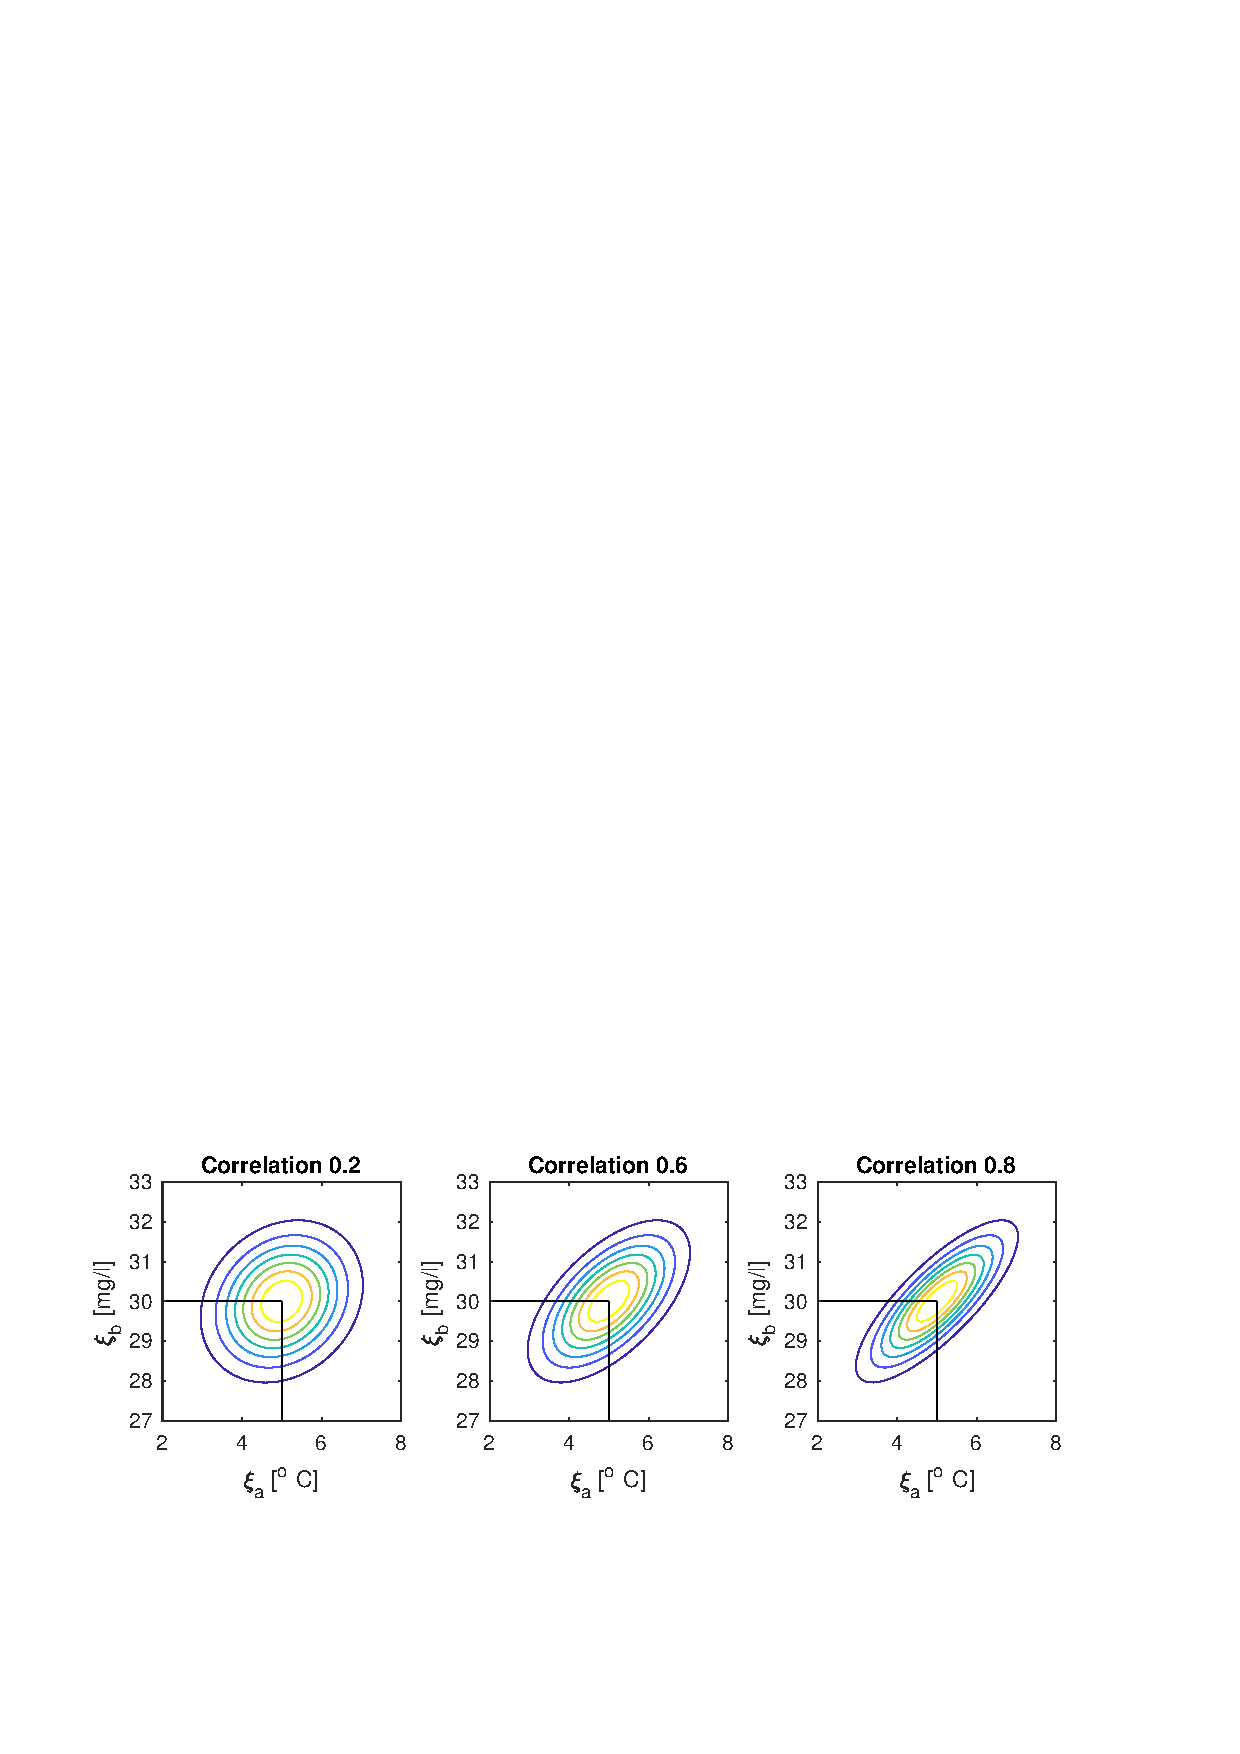
\includegraphics[width=0.99\textwidth]{Figures/illus_bivar.pdf}
  \caption{Density contour plots with different correlations between
    temperature and salinity. The densities have unit variance and the
    thresholds are identical to the mean values $5^o C$ and
    $30 mg/l$. X-axis is temperature and y-axis is salinity.}
\label{illus_bivarDens}
\end{figure}
The displayed densities have unit standard deviations for both
temperature and salinity, but we also study the effect of doubling the
standard deviations.

Table \ref{tab:sim_rhoab} shows the initial EPs and the associated
Bernoulli variance (second row) for the examples indicated in Fig.
\ref{illus_bivarDens}. The EPs increase with the correlation as there
is a strong tendency to have concurrently low temperature and salinity. The Bernoulli variance is similarly large for high
correlations. EPs and Bernoulli variances are the same for standard
deviation $1$ or $2$, which implies that high variability in
temperature and salinity is not captured in the $p(1-p)$ expression.

\begin{table}[!h] \centering \caption{EP and Bernoulli variance for
    different correlations and variances (top rows), and expected
    Bernoulli variances for both temperature and salinity data $\by$ and 
    temperature $y_2$ (bottom rows).}
  \begin{tabular}{c|ccc|ccc}
 &\multicolumn{3}{c}{$\sigma_1=\sigma_2=1$} & \multicolumn{3}{c}{$\sigma_1=\sigma_2=2$} \\
\hline
Correlation $\gamma$ & 0.2 & 0.6 & 0.8 & 0.2 & 0.6 & 0.8 \\
\hline
$p$ & 0.28 & 0.35 & 0.40 & 0.28 & 0.35 & 0.40 \\ 
$p(1-p)$ & 0.20 & 0.23 & 0.24 & 0.20 & 0.23 & 0.24 \\ 
EIBV, Temp and Salinity data & 0.092 & 0.089 & 0.085 & 0.052 & 0.051 & 0.049 \\ 
EIBV, Temperature data only & 0.151 & 0.138 & 0.123 & 0.137 & 0.114 & 0.093 \\ 
\hline
\end{tabular}
\label{tab:sim_rhoab}
\end{table}

Table \ref{tab:sim_rhoab} (bottom two rows) shows results of expected
Bernoulli variance calculations. This is presented for a design
gathering both data types, and for a design with temperature
measurements alone. When both data are gathered, the measurement model is
$(Y_{d,1},Y_{d,2})^t=(Z_1,Z_2)^t+\bepsilon$, with $\bepsilon \sim N(0,0.5^2I_2)$, while $Y_d=Z_1+\epsilon$, $\epsilon \sim N(0,0.5^2)$ when only temperature is measured.
For this illustration, Table \ref{tab:sim_rhoab} shows that the
expected Bernoulli variance gets lower with larger standard deviations
$\sigma_1$ and $\sigma_2$ (right columns). The reduction of Bernoulli
variance is largest for the cases with high correlation
$\gamma$. Albeit smaller, there is also uncertainty reduction when
only temperature is measured (bottom row), especially when temperature
and salinity are highly correlated. When correlation is low
($\gamma=0.2$), there is little information about salinity in the
temperature data, and therefore less uncertainty reduction. In an
application with fresh cold water from a river source, the temperature
and salinity variables will not only be interdependent, but will also
likely show dependence in the spatial dimension. This in turn will
impact the design criteria when we evaluate the information measure by
integrating over several locations (Section \ref{sec:simulations}).

%\subsection{Expected classification criteria}

%{\bf{I have not done anything here - skip this, I think}}.

%Rather than minimizing expected variance one can aim at minimizing the classification probability of the excursion set: 
%$\min [p,(1-p) ]$, see e.g. \cite{lilleborge2016information}. 

%Again, since the conditional mean is a linear in the data, we only have to look at the %relevant linear combination via $\bm_{\xi}=E(\bxi)$.
%See also \cite{bhattacharjya2013value}.

%\begin{equation}
%E(\min \{ p,(1-p)\})=\int \min P(\xi_1 \leq t, \xi_2 \leq s),[1-P(\xi_1 \leq t, \xi_2 \leq s)] p(E(\bxi)=) dE(\bxi)=,
%\end{equation}
%for the complementary probabilities, this is again evaluated by the corner regions for the block, and $\Phi_4()$ evaluations are required.

%In the end, this result is integrated over the spatial domain $x \in X$.